\section{ПОГРАМНА РЕАЛІЗАЦІЯ}

\subsection{Парадигма програмування та архітектура}
Програмний код був написаний мовою Python. Оскільки це мультипарадигменна мова програмування,
у застосунку було використано як імперативний об'єктно-орієнтований так і функціональний підходи.
У вигляді ООП класів представлена інформаційна модель, тобто основна структура
даних - дерево та її складові. До функціональної парадигми можна віднести методи обробки
дерев. Оскільки дерева це рекурсивні структури, широко використовувалася рекурсія.
Було підключено всього дві сторонні бібліотеки на мові Python: conllu - для парсингу розміченого
корпусу та pandas - бібліотека, яка полегшує роботу зі статистикою та аналізом даних.

Умовно, програму можна розбити на 3 частини. Перша відповідає за нормалізацію
юнікоду та парсинг вхідного файлу. Не завжди на вхід може прийти правильно
закодований файл, тому необхідно привести його до того вигляду, щоб парсер без
перешкод міг зчитати всю інформацію. Цей модуль по суті відповідає за зчитування
файлу з жорсткого диску та завантаження його до оперативної пам'яті. Друга частина
програми відповідає за збір даних із завантаженого файлу. Дуже важливо використовувати
правильні структури даних адже тільки у певній репрезентації можна знайти необхідну
інформацію. В цій частині як основні структури даних використовувалися
списки дерев та інші допоміжні класи такі як Signature, які реалізовані із застосуванням ООП.
Третьою частиною можна вважати аналізатор цих зібраних даних.

\begin{figure}[p]
  \begin{center}
    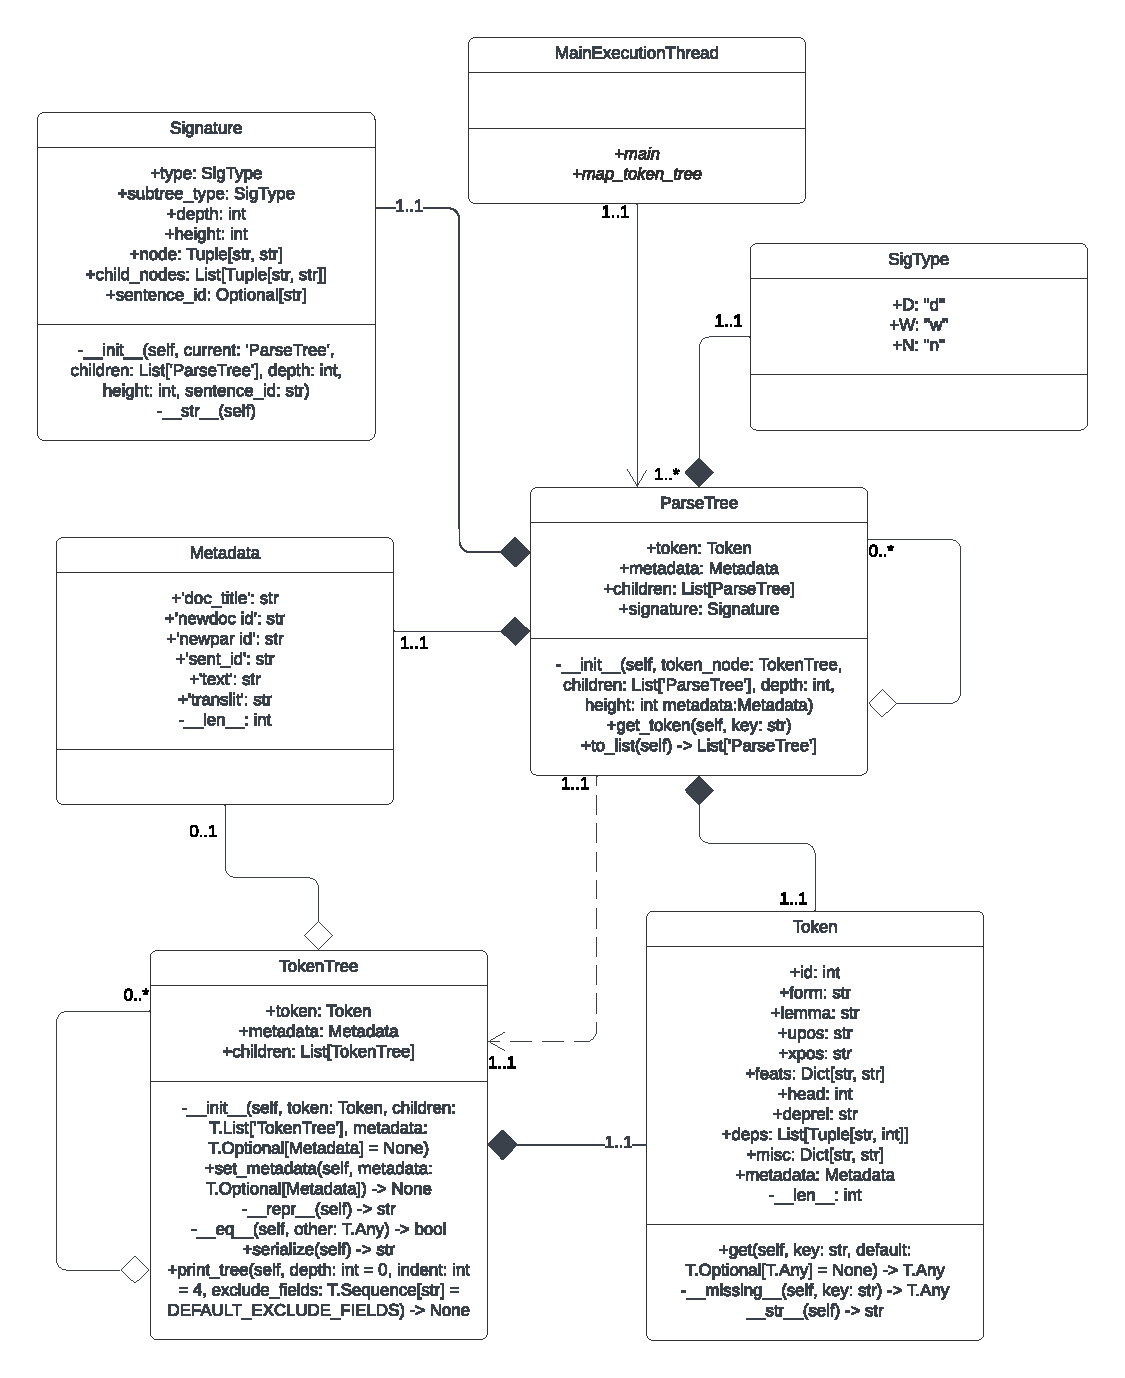
\includegraphics[width=0.9\textwidth]{ud_class_diagram.pdf}
  \end{center}
  \caption{Діаграма класів моделі корпусу}
  \label{img:class_diagram}
\end{figure}
\newpage

На рисунку \ref{img:class_diagram} зображені відношення класів моделі одне до одного.
Як можна побачити звідси, головним класом є ParseTree, який залежить від інших класів
в основному відношенням композиції. Також звідси видно, що дерево є рекурсивною
структурою адже посилається саме на себе.

Даний застосунок не потребує графічного інтерфейсу. Всі операції можливо здійснити
через командний рядок. Також, скрипти на мові Python легко редагувати тому що вони не
потребують повторної компіляції, тому змінити необхідні параметри можна в тому
числі і у вихідних файлах з кодом. Доступ до файлів розбору здійснюється
також за допомогою командного рядка. Досить лише клонувати репозиторій із
банками дерев і вказати до нього шлях у файловій системі. Оскільки застосунок
чітко не прив'язаний до даних, які потрібно аналізувати, можна використовувати будь-які
дані, які задовольняють наступним вимогам.

\begin{enumerate}
    \item на вхід повинні подаватися звичайні текстові файли
    \item ці файли повинні задовольняти усім вимогам CoNLL-U
\end{enumerate}

У ході роботи було розроблено діаграму прецедентів, рисунок \ref{img:use_case_diagram}.
По якій можна детальніше ознайомитися із прикладами використання програми.

\begin{figure}[p]
  \begin{center}
    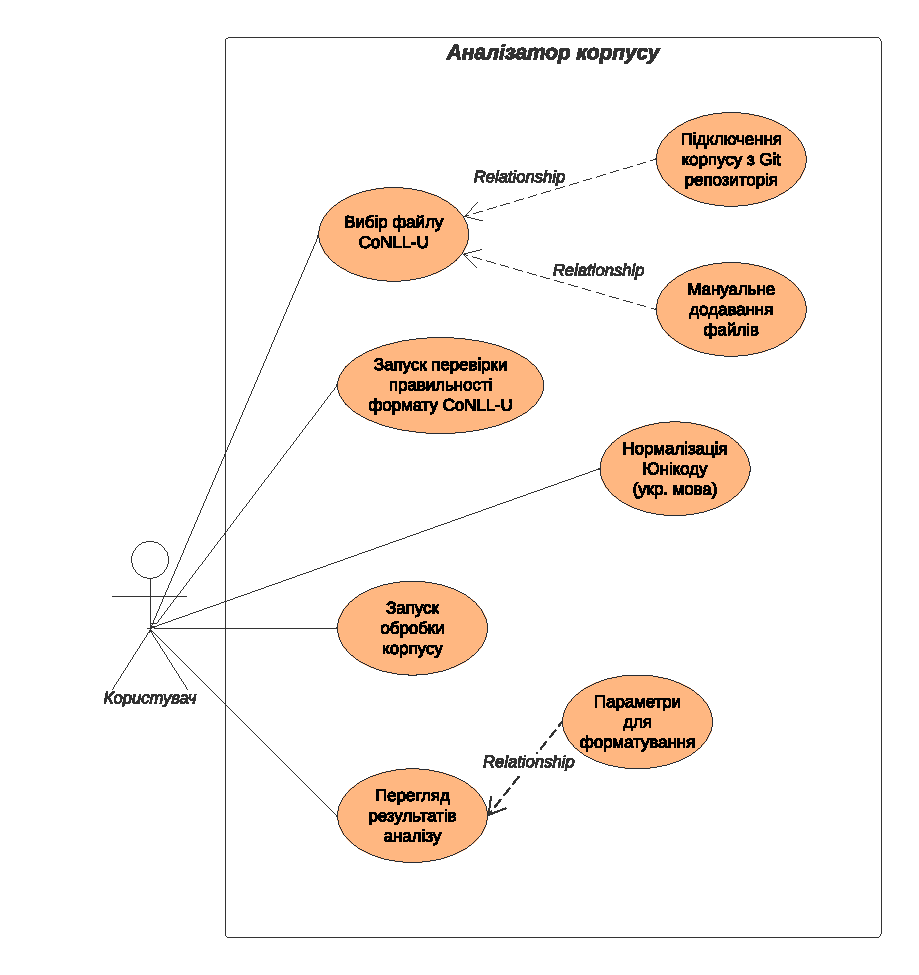
\includegraphics[width=0.9\linewidth]{ud-use-case-diagram.pdf}
  \end{center}
  \caption{Діаграма прецеденнтів аналізатора корпусу текстів}
  \label{img:use_case_diagram}
\end{figure}
\newpage

\subsubsection{Модуль типізації}
Як доповнення до типізації мови Python, яка є одночасно сильною, тобто не дозволяється змінювати
тип ідентифікатора після його першого присвоювання, та динамічною, тобто тип ідентифікатора
може бути визначений після його оголошення, використовувався модуль типізації зі стандартної
бібліотеки typings. Який дозволяє писати код, схожий,
як у статично-типізованих мовах, наприклад Java.
Єдиним недоліком явного вказування типів є те, що це в якійсь мірі уповільнює розробку, коли
розмір проетку не перевищує декількасот рядків коду. Але у такого підходу є і ряд переваг.
По-перше, програмний код стає зрозумілішим, тому що не доводиться припускати або здогадуватися
із контексту що насправді знаходиться у змінній. Написання значущих імен для ідентифікаторів
в якійсь мірі вирішує цю проблему, але коли мова йде про якусь специфічну область розробки,
наприклад парсинг файлу типу CoNLL-U, то людині, яка глибоко не розбирається у цій темі,
ім'я ідентифікатору не буде ні про що говорити (наприклад імена UPOS та DEPREL стають трохи
зрозумілішими, якщо видно, що вони типу String). По друге, сучасні інструменти розробки
використовують протокол Language Server Protocol \cite{bib4}, розроблений компанією Microsoft,
який дозволяє уніфікувати взаємодію між мовами програмування та редактором коду. Внаслідок
чого, середовища розробки мають змогу пропонувати різні дії з кодом (наприклад автоматично
імпортувати програмні модулі) та ``підсвічувати'' типи і пропонувати автодоповнення, що в рази
спрощує та пришвидшує процес написання коду. У цій роботі, як допоміжний інструмент
використовувався мовний сервер Pyright, який автоматично поставляється в середовищі PyCharm.
Із використаним модулем типізації, Pyright пропонує більш точні підказки для автодоповнення
адже йому самому не портібно виводити типи із контексту, він використовує уже статично оголошені.
Все це сприяє підвищенню зрозумілості кодової бази і з розростанням проекту дозволяє не
запам'ятовувати що знаходиться у кожній змінній, а покладатися на підказки мовного сервера.

\subsubsection{Модуль тестування}
Для підвищення надійності та коректності програми використовувався підхід модульного
тестування. Мова Python пропонує модуль зі стандартної бібліотеки під назаою unittest.
Завдяки ньому, можна створити окрему вхідну точку в програму, запустити і протестувати її,
при цьому не модифікуючи складових цієї програми.

\begin{figure}[ht]
  \begin{center}
    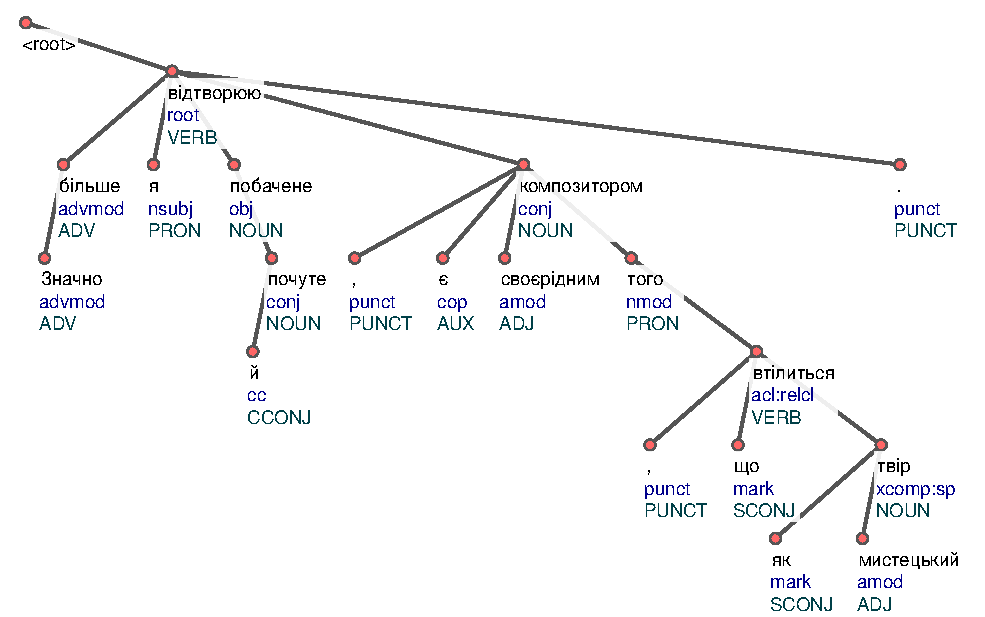
\includegraphics[width=0.9\linewidth]{conllu_tree.pdf}
  \end{center}
  \caption{Протестоване дерево}
  \label{img:tested_conllu_tree}
\end{figure}

У ході роботи було повністю протестовано клас ParseTree \ref{img:class_diagram}, який залежить
від модулів Signature, Metadata та Token. Отже можна гарантувати і коректність роботи цих
модулів. Тести охоплюють функціонал завантаження розпарсованих даних до дерева, доповнення
кожної вершини дерева інформацією про висотою та глибину та додавання до кожної
вершини метаданих, таких як ідентифікатор речення, номер слова у реченні, універсальний тег
частини мови та універсальне відношення залежності до кореневого елементу речення.
На вхід подавалося речення \texttt{"Значно більше я відтворюю побачене й почуте , є своєрідним
композитором того , що втілиться як мистецький твір ."}, рисунок \ref{img:tested_conllu_tree}.
Наприклад, для слова \texttt{"відтворюю"} кінцева сигнатура гарантовано буде
\texttt{"w(root+VERB, advmod+ADV, nsubj+PRON, obj+NOUN, conj+NOUN, punct+PUNCT, 5, 0, 5, 2hkl)"}.
Оскільки це коренева вершина, її відношення до кореневого елементу вказане як \texttt{"root"}
та глибина дорівнює нулю. Ця вершина має 5 прямих нащадків та висоту дерева 5 одиниць. Ми можемо
переконатися у правильності цього, поглянувши на рисунок \ref{img:tested_conllu_tree}.

\subsection{Структури даних}
Як основна струтура даних використовувалося дерево, на основі якого збиралися необхідні
для аналізу дані. Як допоміжні структури використовувалися асоціативні масиви, списки та
кортежі.

Найефективніими по об'єму пам'яті є кортежі та списки адже в цих структурах зберігається
мінімум допоміжної інформації, такої, як вказівники на нащадків. Кортежі та списки - це
в чомусь схожі структури даних адже обидві призначені для зберігання колекцій даних.
Обидві є гетерогенними структурами, тобто можуть зберігати будь який тип даних.
Обидві є послідовними структурами, тобто можна ітерувати по елементам, які містяться в
цих структурах. Та що у списках що в кортежах можна доступатися до елементів за порядковим
номером. Але ключовою відмінністю є те, що кортежі, на відміну від списків не можна
модифікувати після оголошення. Це робить кортежі більш ефективними адже інтерпритатору
Python не доводиться виділяти додаткову пам'ять під час роботи програми.
У програмі кортежі використовувалися для зберігання саме таких даних, які не будуть
змінюватися з часом, наприклад універсальний тег частини мови та
універсальне відношення залежності до кореневого елементу речення для сигнатур
вершин дерев. Дійсно, такі дані є невід'ємною частиною сигнатури, тим паче що
оголошені ще у вихідному файлі з корпусу текстів. У вигляді списків зберігалися
нащадки вершини дерева. Незважаючи на те, що ці дані теж відомі заздалегідь та
знаходяться в корпусі, через особливості рекурсивного обходу дерева, яке відбувається
у глибину, неможливо ініціалізувати кортеж із усіх нащадків вершини адже
такий обхід передбачає додавання по одному нащадку за одну рекурсивну ітерацію.
Тобто передбачається, що розмір структури даних повинен збільшуватися із подвльшим
ітеруванням по нащадкам. Також є функція розкладання у вигляді списку дерева токенів,
що робить таку структуру більш ефективною по розміру пам'яті, але втрачаются усі
корисні властивості дерев. Основним недоліком списків та кортежів є те, що операції
з пошуку елементів здійснюются за лінійним часом $O(n)$, що є неефективним зі
зростанням кількості елементів. Але у програмі не застосовувалися алгоритми
пошуку для вузлів дерев, тому таким недоліком можна знехтувати.

Асоціативні масиви або хеш-таблиці використовувалися для зберігання пар ``ключ-значення''.
У асоціативному масиві гарантовано зберігаються унікальні ключі, таким чином кожен 
можливий ключ з’являється в колекції не більше одного разу. Ця структура даних
використовувалася для записування таких даних як \texttt{id, form, lemma, upos, xpos,
feats, head, deprel, deps, misc} для кожного токена слова та метаданих для кожного
речення. У об'єктно-орієнтованому підході цю структуру
можна було б замінити класом але такий клас не містив би в собі
методів обробки цих даних. До того ж, довелося б визначати методи доступу для кожного
поля, так звані ``геттери'' та ``сеттери''. Написання такого коду негативно
вплинуло б на зрозумілість програми адже важко з першого погляду відокремити
шаблонний код від того, який дійсно несе в собі корисне смислове навантаження.
Хеш-таблиці позбавлені такого недоліку, тому що вони мають один метод доступу
до всіх даних, які в собі містять. Потрібно лише вказати ключ доступу, який зазвичай
є типу \texttt{String}. У разі якщо такий ключ міститься в таблиці, цей метод поверне
його значення. Якщо ж такого ключа немає, то повернеться пусте значення. Крім того,
хеш-таблиці зазвичай мають функції, окрім доступу до значеннь, також додавання
та видалення цих значеннь. Якщо використовувати замість цього клас, ці методи довелося б
реалізовувати для кожного з полів. Зазвичай хеш-таблиці реалізовані за допомогою
інших двох структур - це уже згаданих списків та червоно-чорних дерев, в яких дані
зберігаються за хеш-сумою та оптимізуюются для вставки та видалення. Тому операції
з пошуку, які активно застосовувалися, працюють швидше, аніж у невідсортованих
списках, а саме за логарифмічний час $O(log(n))$.

Усі слова речення та їх токени зберігалися у вигляді дерева. Дерево є найбільш
природньою структурою даних для такої задачі адже дозвляє показати зв'язки
та залежності елементів у вигляді ієрархії. У розміченому файлі типу CoNLL-U дані зберігаются
у вигляді таблиць із чітко заданими розділювальними символами.
У кожного слова анотованого речення корпусу є поле \texttt{deprel},
на основі якого і можна побудувати дерево. Адже це поле показує відношення до кореневого
елементу речення. Крім того, дерева мають інші корисні властивості. Для кожної вершини
можна знайти висоту, тобто шлях від поточної вершини до найглибшого нащадка та глибину,
тобто, шлях від поточної вершини до кореневої вершини дерева.

\begin{center}
    ...todo...
\end{center}

\subsection{Алгоритм виконання}
Програма має чіткий початок та кінець своєї роботи. Вхідна точка \texttt{main()} може
бути викликана через командний рядок. Саме через командний рядок і можна вказати бажаний
для аналізу файл. Вивід інформації також відбувається за допомогою командного
рядка. На вхід необхідно передати шлях до файлу. Програма може завершитися не успішно
тільки у двох випадках: на вхід передано шлях до файлу, якого не існує, або такий
файл не задовольняє вимогам формату CoNLL-U.

Оскільки на вхід передається звичайний текстовий файл, єдина корисна інформація,
яку можна з'ясувати на цьому етапі - це довжина цього файлу. Тому наступним кроком буде
парсинг вмісту до структурних одиниць мови програмування. Спочатку парсер розбиває
файл на рядки, оскільки формат CoNLL-U влаштований таким чином що всі токени слів
містяться на окремих рядках. Ці рядки можуть містити або метадані, або безпосередньо
слова з токенами, або можеть не містити нічого, що слугує індикацією про те, що
речення закінчилося і починається нове. Цей етап парсингу виділяє із кожного рядка
весь вміст і на виході ми отримуємо двовимірний список токенів. Вкладені
списки є нічим іншим, як реченнями де найменшою одиницею є клас Token,
рис \ref{img:class_diagram}. Далі зазначений список необхідно перетворити у список дерев,
тобто потрібно зробити так, щоб кожне речення постало у формі дерева.
Це робиться за допомогою поля \texttt{deprel}. Створені дерева ще не задовольняють
усім вимогам адже для аналізу потрібно порахувати висоту та глибину для кожної вершини.

\begin{center}
    ...todo...
\end{center}

Фінальним етапом роботи програми є вивід порахованої інформації на екран.

У ході роботи було побудовано діаграму послідовностей, рис \ref{img:sequence_diagram}.

\begin{figure}[p]
  \begin{center}
    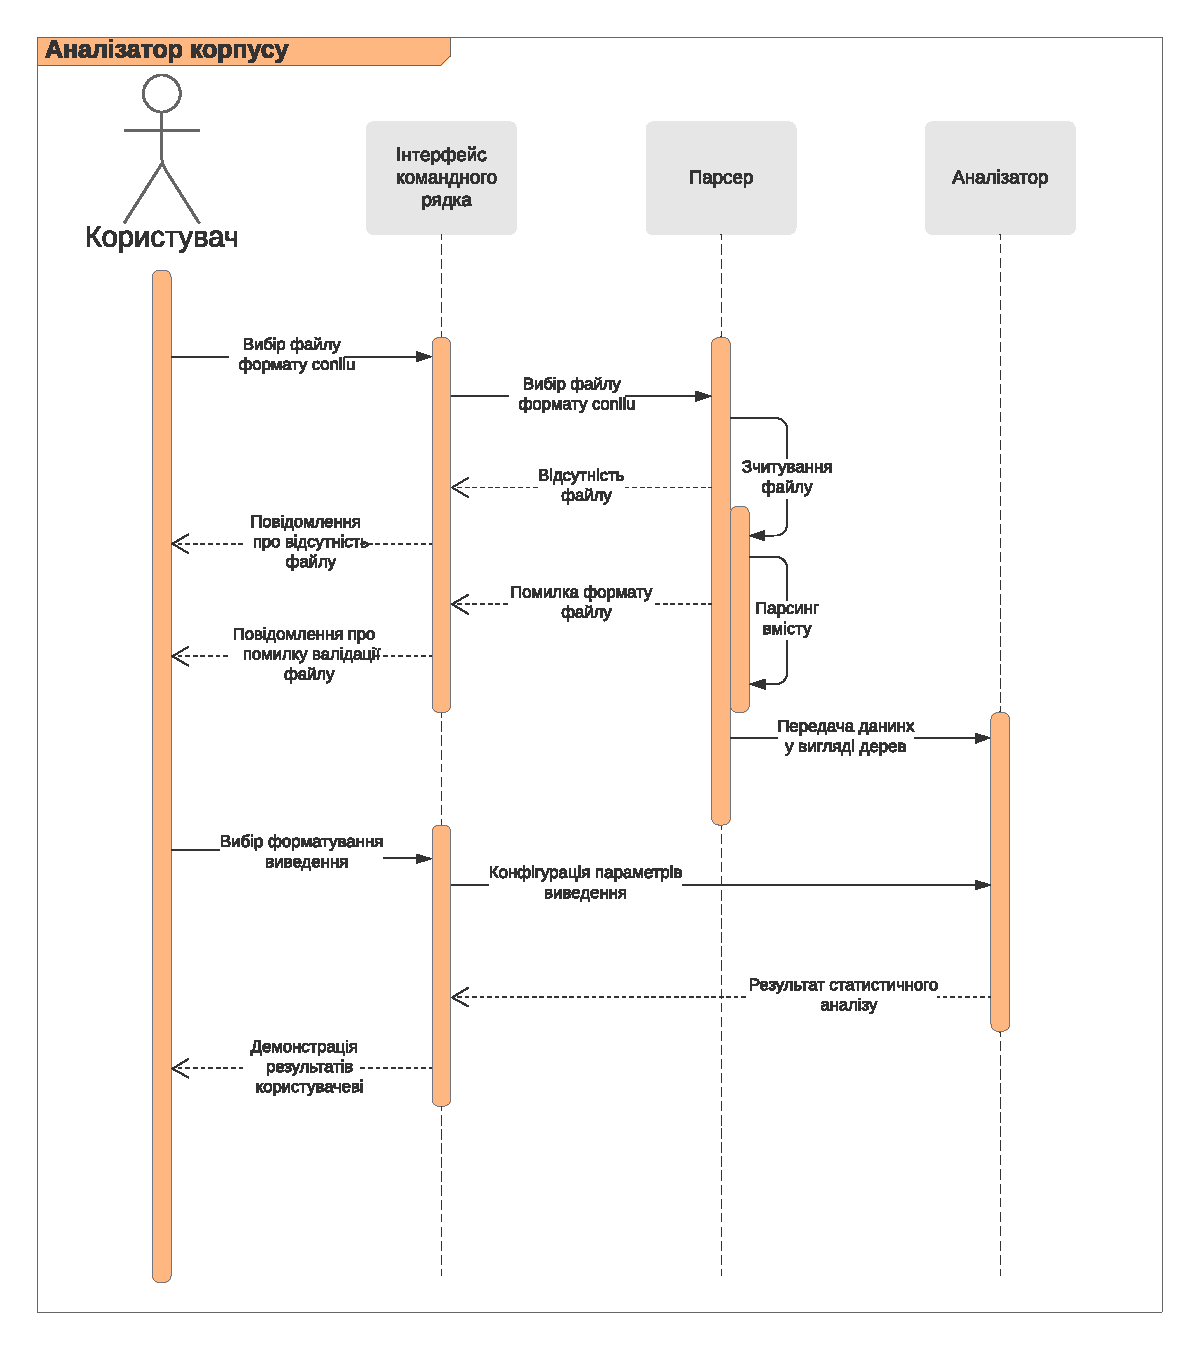
\includegraphics[width=0.9\linewidth]{ud-sequence-diagram.pdf}
  \end{center}
  \caption{Діаграма послідовностей аналізу корпусу текстів}
  \label{img:sequence_diagram}
\end{figure}
\newpage


